\section{算例 1：无限大母线}
\label{sec:ex_1}
本节研究如何应用所提方法分析变流器接入前述无限大母线系统时的稳定性。此外，我们还讨论第~\ref{sec:lim} 节所示的保守性问题，以及如何通过适当选择权重矩阵 $W_i(s)$ 缓解这一问题。

\subsection{虚拟导纳补偿}
图~\ref{fig:GFM_gain_phase_test} 表明，即使两个系统都具有扇形性，小相位特征值界在 $50$ Hz 以下仍然非常保守。其原因是 $Y_C$ 和 $Y_{net}^{-1}$ 都具有较大的相位范围。回顾式~\eqref{eq:phase_bound}，小相位界采用最坏情况组合，即最大值与最大值配对、最小值与最小值配对。然而，在乘积 $Y_CY_{net}^{-1}$ 中可能出现有利的相位相互作用，产生部分抵消并减小其特征值相位。图~\ref{fig:phase-bounds_Yv} 清楚展示了这一现象：小相位界 $\Phi(Y_C)+\Phi(Y_{net}^{-1})$ 明显高估了实际特征值相位 $\angle\lambda(Y_CY_{net}^{-1})$。

\begin{figure}
\centering
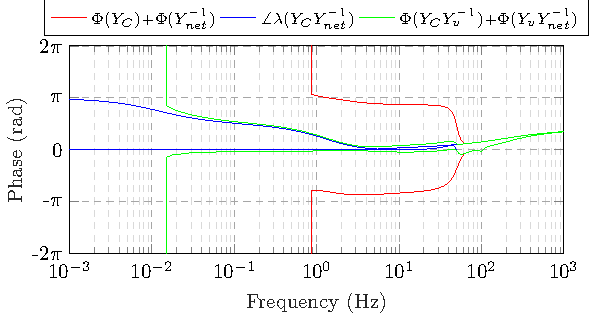
\includegraphics[width=\linewidth]{Phase_Bounds.pdf}
\caption{采用虚拟导纳补偿前后的小相位界。}
\label{fig:phase-bounds_Yv}
\end{figure}

减小数值域的相位张角、限制极端相位组合，可以获得更紧的界。由于变流器实现了虚拟导纳控制 $Y_v(s)$，且其约 $50$ Hz 附近的行为主要由虚拟导纳决定，可以将 $Y_C(s)$ 右乘 $Y_v(s)^{-1}$，使该频段内 $Y_C(s)Y_v(s)^{-1}\approx I$。网络导纳也相应变换为 $Y_{net}(s)Y_v(s)^{-1}$。从另一角度看，这相当于把一项已知动态特性从变流器转移到网络，从而降低保守性。在式~\eqref{eq:freq_dep_tf_better} 中，对应于选择 $W_i(s)=Y_v(s)^{-1}$。

图~\ref{fig:phase-bounds_Yv} 展示了补偿效果。采用所提虚拟导纳滤波后，相位界得到明显改善。乍看之下，这似乎会破坏认证的分散性；但在实践中并不需要精确知道虚拟导纳数值（即约 $50$ Hz 附近的行为），后文将表明近似值已经足够。在分散式场景中，这些数值既可预先选为固定参数，也可由稳定性认证方为不同装置分别指定。无论如何，拟议中的 GFM 并网规范已经给出了有效阻抗的固定范围~\cite{entsoe}。

\begin{rem}
图~\ref{fig:phase-bounds_Yv} 显示，当频率趋于零时，一个特征值的相位趋近 $\pi$。在该频段，小增益条件不能保证 $|\lambda|<1$，稳定性评估因而没有结论。这说明需要引入 $\mathcal{C}$ 所产生的平移，将开环传递函数的特征值移到更合适、可由小相位条件认证稳定性的区域。
\end{rem}

\subsection{完整变换}
图~\ref{fig:phase-dep-frame} 给出了采用频率相关变换~\eqref{eq:generic_trasnf} 后的小相位判据结果，其中矩阵按式~\eqref{eq:freq_dep_tf_better} 定义，滤波器截止频率设为 $0.5$ Hz。与此前结果相比，系统在整个频率范围内都能保持扇形性，并且仅凭小相位条件即可保证闭环稳定。

这意味着该 GFM 变流器的稳定性不依赖以增益衡量的电网强度，在强网和弱网条件下都能保持稳定。从这个意义上说，小相位条件提供了与电网强度无关的稳定性保证。但网络特性变化（如 $R/X$ 比或负荷水平改变）会改变网络相位，可能减小相位裕度并推动变流器趋于失稳。

\begin{figure}
\centering
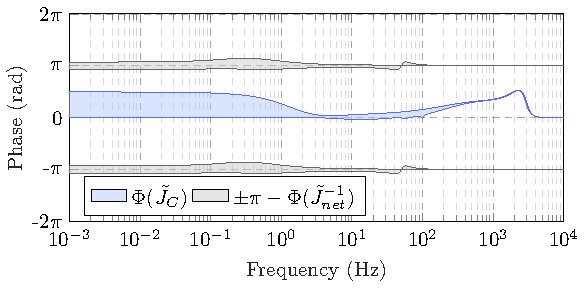
\includegraphics[width=\linewidth]{Phase_mixed.pdf}
\caption{采用式~\eqref{eq:generic_trasnf}、\eqref{eq:freq_dep_tf_better} 的频率相关变换后，GFM 变流器的小相位条件。}
\label{fig:phase-dep-frame}
\end{figure}

\subsection{不稳定情形}
为进一步验证该方法，下面考察定理充分条件的逆否命题：若闭环系统不稳定，则必存在某个频率，使小相位和小增益条件同时被违反。实践中，要使 GFM 变流器失稳并不容易。按照文献~\cite{de2012automatic}，我们在公共耦合点接入纯电阻负载并增大无限大母线阻抗。将控制模式切换为恒无功功率（恒 Q），并把 GFM 的 VSM 阻尼从 $0.5$ 降至 $0.05$ 后，闭环系统失稳，出现 $1.2$ Hz 的持续振荡。图~\ref{fig:GFM_Unstable} 给出了采用所提变换后的混合增益/相位检验结果。

启用无功功率控制会降低低频增益，使小增益条件得到满足。然而，稳定情形（$D=0.5$）满足小相位条件；不稳定情形（$D=0.05$）中，变流器相位显著增大，并与网络相位共同导致相位条件被违反，同时在不稳定振荡频率附近也不满足增益条件。

\begin{figure}
\centering
\begin{subfigure}{\columnwidth}
  \centering
  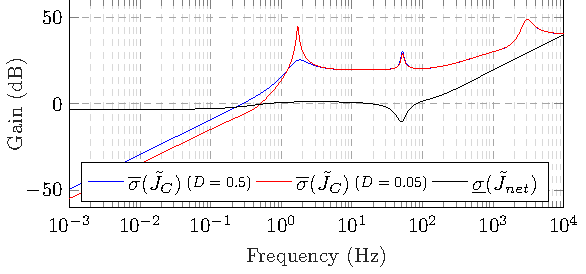
\includegraphics[width=\linewidth]{Gain_inf_un.pdf}
\end{subfigure}
\begin{subfigure}{\columnwidth}
  \centering
  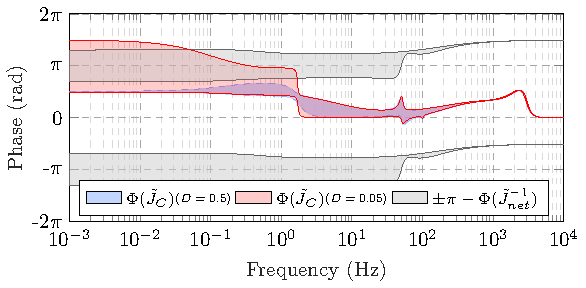
\includegraphics[width=\linewidth]{Phase_inf_un.pdf}
\end{subfigure}
\caption{GFM 接入无限大母线：稳定（$D=0.5$）与不稳定（$D=0.05$）情形对比。}
\label{fig:GFM_Unstable}
\end{figure}

\section{算例 2：IEEE 14 节点系统}
\label{sec:ex_2}
\begin{figure}
\centering
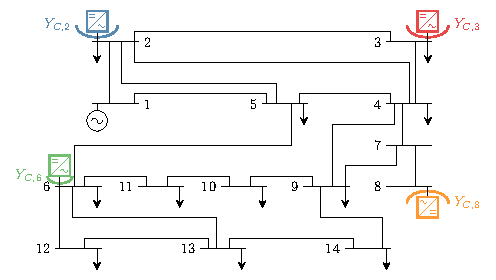
\includegraphics[width=\linewidth]{IEEE14_diagram.pdf}
\caption{IEEE 14 节点系统示意图。}
\label{fig:ieee14_diagram}
\end{figure}

为进一步验证所提方法的可扩展性，本文采用图~\ref{fig:ieee14_diagram} 所示的改进 IEEE 14 节点系统，其参数见文献~\cite{RepoZenodo}。四台 GFM 变流器分别接入节点 2、3、6 和 8。

与无限大母线算例类似，为构造不稳定情形，将变流器 8 的阻尼设为较低值，接入纯电阻负载，并增大线路 7--8 的阻抗。在该配置下，系统发生由变流器 8 驱动的 $0.54$ Hz 不稳定振荡。图~\ref{fig:IEEE14_criteria} 给出了采用所提变换和虚拟导纳补偿后的分散式条件。变流器 2、3 和 6 满足小相位条件，而变流器 8 不满足；具体而言，在 $1.64$ Hz 以下，其相位与网络相位发生重叠。相位重叠本身并不能推出系统不稳定；但在已知系统失稳的情况下，该结果可以识别责任变流器，并可通过适当重调其控制参数恢复稳定。例如，将满足小相位条件的变流器 6 的整定参数用于变流器 8 后，系统即可恢复稳定。

本算例中，各变流器采用不同的虚拟导纳 $R/X$ 比，如表~\ref{tab:virt_adm} 所示；但所有变流器的虚拟导纳补偿均采用固定值 $R_v=0.01$、$X_v=0.1$。这表明即使不知道精确的虚拟导纳，只要采用合理估计，仍可获得适当的相位界，并利用所提方法有效验证稳定性。

\begin{figure}
\centering
\begin{subfigure}{\columnwidth}
  \centering
  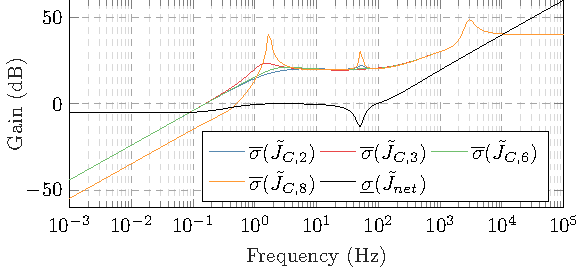
\includegraphics[width=\linewidth]{Gain_14.pdf}
\end{subfigure}
\begin{subfigure}{\columnwidth}
  \centering
  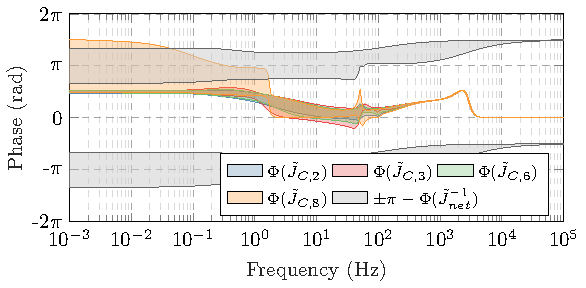
\includegraphics[width=\linewidth]{Phase_14.pdf}
\end{subfigure}
\caption{IEEE 14 节点系统的稳定性分析。}
\label{fig:IEEE14_criteria}
\end{figure}

\begin{table}
\centering
\caption{IEEE 14 节点系统中的虚拟导纳设置。}
\label{tab:virt_adm}
\begin{tabular}{ccc}
GFM 节点 & $R_v$（p.u.） & $X_v$（p.u.）\\
\hline
$2$ & $0.02$ & $0.1$\\
$3$ & $0.05$ & $0.1$\\
$6$ & $0.03$ & $0.1$\\
$8$ & $0.01$ & $0.1$\\
\hline
\end{tabular}
\end{table}
